\paragraph{OpenWhisk Evaluation Function Details.}


% The impact on the different function performances can be seen in Figure~\ref{fig:faasbench}.
% For this figure, to generate the workload, the first three functions have an inter-arrival time of 1500 ms, and the fourth (floating-point) has a lower IAT of 400 ms. 


We use the following functions from FunctionBench FaaS benchmark to run on OpenWhisk. 

\begin{enumerate}
  \item ML Inference: Image inference using the SqueezeNet CNN architecture, implemented in Tensorflow.
  \item Video Encoding: Download 11 MB mp4 file and convert it to a grayscale avi equivalent, using Python's cv2. 
  \item Matrix Multiplication: Using Numpy and \texttt{linalg.solve} of a randomly generated 20x20 matrix.
  \item Disk-bench: Read and write 1000 times from disk in 128k blocks using the \textbf{dd} command
  \item Web-serving: Generating and returning HTML for a small web page using Python's Chameleon. 
  \item Floating Point: A series of floating point trigonomotric computations using the standard Python math library.
\end{enumerate}



\paragraph{Azure Functions Dataset.}

We use the Azure function dataset to validate our keep-alive policies.
The full dataset consists of 14 days of function invocations, and billions of individual invocations. 
We use the first day's data, and do not consider functions with less than two invocations. 

Because memory is tracked at the \textit{application} level, and applications are made up of multiple functions, we evenly split the memory allocation between all functions in an application.


The dataset provides invocations in minute-wide buckets.
So when forming the traces, if there is only one invocation it is injected at the beginning of the minute.
For multiple invocations, they are equally spaced throughout the minute.

%Dataset location: https://github.com/Azure/AzurePublicDataset/blob/master/AzureFunctionsDataset2019.md

We use multiple different samples of this trace to validate our approach with different kinds of traces, and to make the analysis more tractable. We note that the full function trace is suitable for a large cluster of servers, whereas our focus is on a \emph{single} server.
The details of our trace samples are provided in Table~\ref{tab:trace-deets}. 
Figure~\ref{fig:whole-trace} shows the invocations/second of the full function trace (without sampling), and Figures~\ref{fig:392-trace}, \ref{fig:1000-trace}, and \ref{fig:200-trace} show the timeseries of our three workload traces. 
We can see that the representative trace (Figure~\ref{fig:392-trace}) captures the diurnal effects seen in the full trace (Figure~\ref{fig:whole-trace}).



\begin{table}
  \begin{tabular}{lrrr}
    \hline 
    Trace & Num Invocations & Reqs per sec & Avg. IAT \\
    \hline
    Representative & 1,348,162 & 190 /s & 5.4 ms \\
    Rare & 202,121 & 30 /s & 36 ms \\
    Random & 4,291,250 & 600 /s & 1.8 ms \\
    \hline
  \end{tabular}
  \caption{Size and IAT details for the three traces used in our evaluation.}
  \label{tab:trace-deets}
\end{table}


\begin{comment}

\begin{figure}[t]
  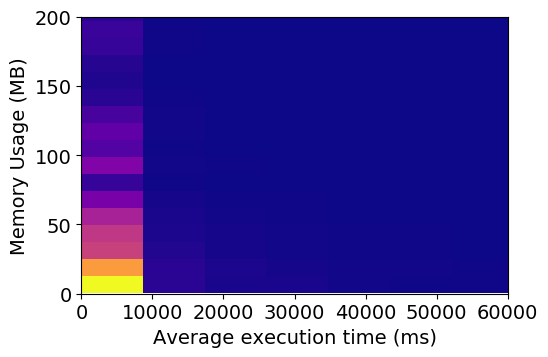
\includegraphics[width=0.3\textwidth]{../graphs/azure_analysis/mem-dur-corr.png}}
  \caption{Lack of correlation between a function's memory and average runtime duration}
  \label{fig:azure-mem-dur-corr}
\end{figure}

\begin{figure}[t]
  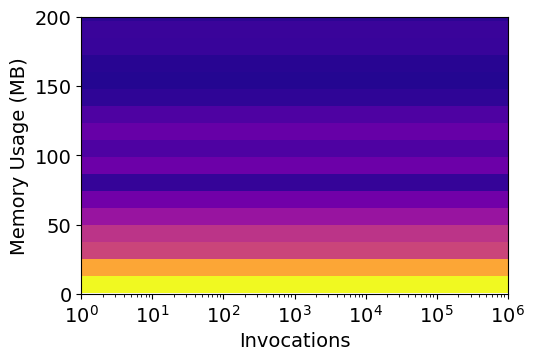
\includegraphics[width=0.3\textwidth]{../graphs/azure_analysis/mem-conv-corr.png}
  \caption{Lack of correlation between a function's memory and number of  times it is invoked}
  \label{fig:mem-invok-corr}
\end{figure}

\begin{figure}
    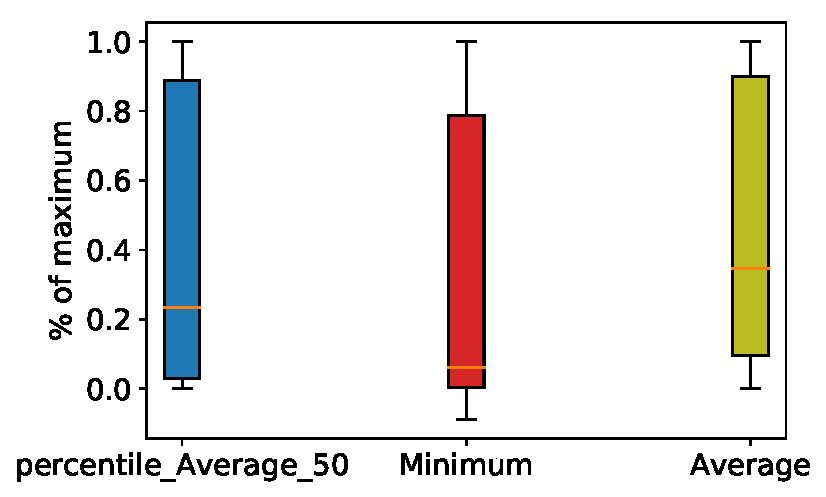
\includegraphics[width=0.3\textwidth]{../graphs/azure_analysis/cold_vs_warm.pdf}
    \caption{Relation between a functions maximum runtime and it's minimum, average, and 50th percentile average.}
    \label{fig:warm-cold-box}
\end{figure}

\end{comment}

\begin{figure}
 \centering 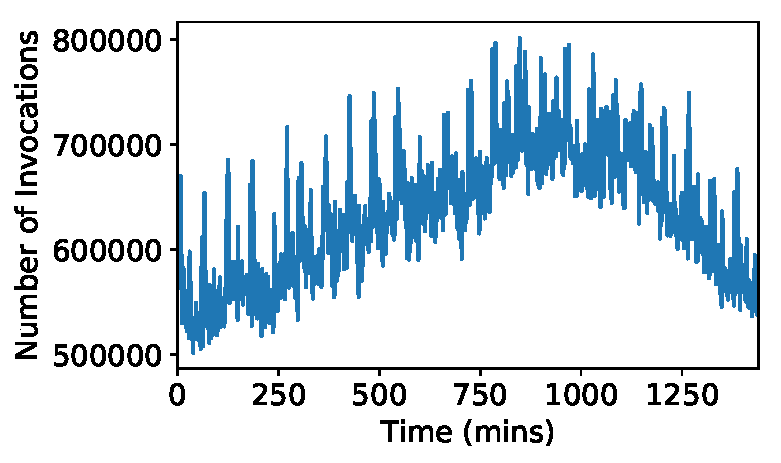
\includegraphics[width=0.3\textwidth]{../graphs/azure_analysis/whole_trace.pdf}
  \caption{Full Azure trace (Day 1) invocation timeseries.}
  \label{fig:whole-trace}
\end{figure}


\begin{figure}
 \centering   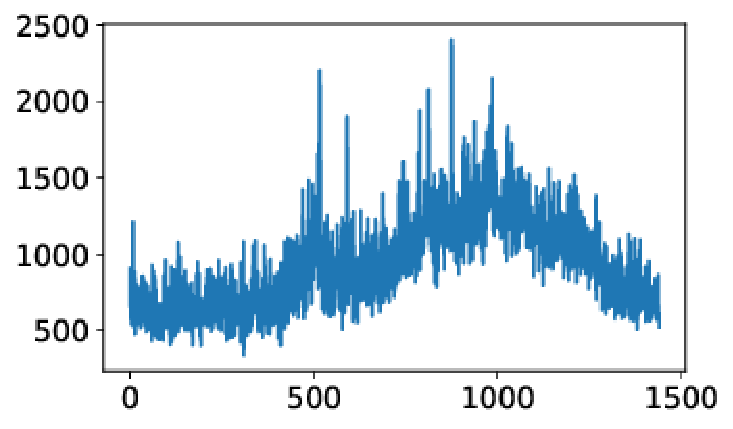
\includegraphics[width=0.3\textwidth]{../graphs/rep-funcs-392/392-b-trace.pdf}
  \caption{Representative trace invocation timeseries.}
  \label{fig:392-trace}
\end{figure}

\begin{figure}
  \centering  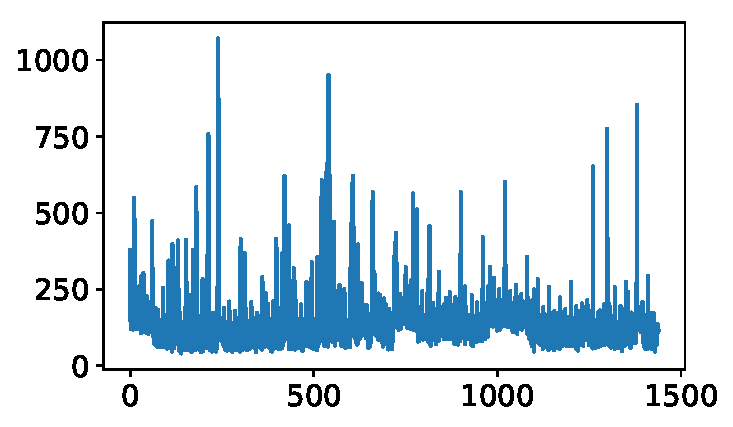
\includegraphics[width=0.3\textwidth]{../graphs/rare-funcs-1000/1000-b.pdf}
  \caption{Rare function trace invocation timeseries.}
  \label{fig:1000-trace}
\end{figure}


\begin{figure}
  \centering  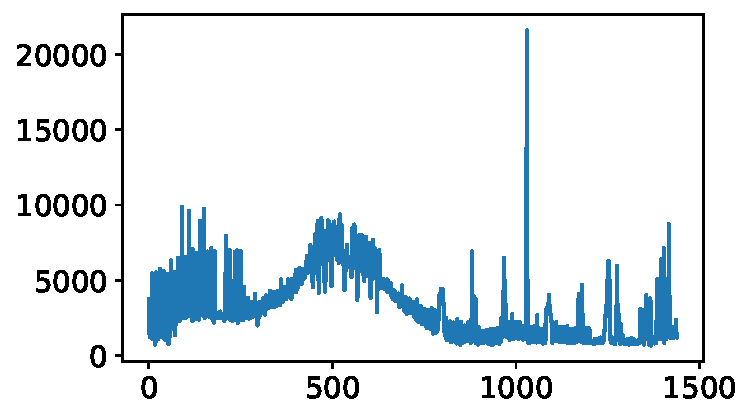
\includegraphics[width=0.3\textwidth]{../graphs/random-funcs-200/200-c.pdf}
  \caption{Randomly sampled trace invocation timeseries.}
  \label{fig:200-trace}
\end{figure}

%\end{comment}

%%% Local Variables:
%%% mode: latex
%%% TeX-master: "appendix-submit"
%%% End:
